\documentclass[11pt]{article}

\usepackage{thumbpdf, amssymb, amsmath, amsthm, microtype,
	    graphicx, verbatim, listings, color, fancybox}
\usepackage[pdftex]{hyperref}
%\usepackage[margin=1in]{geometry}
\usepackage{cawsty}
\usepackage{fullpage}
\usepackage{pseudocode}
\usepackage{fancybox, fancyvrb}

\newcommand{\field}[1]{\mathbb{#1}} %requires amsfonts

%\setlength{\parindent}{0pt}

\linespread{0.9}

\begin{document}
\cawtitlelong{4040-849 Optimization Methods}{Optimizing Cryptographic Strength of Substitution}{Layers in Symmetric-Key Cryptosystems}

\begin{abstract}
The cryptographic security of symmetric-key cryptosystems is based upon Shannon's principles of confusion and diffusion \cite{Kim90astudy}. Confusion can be defined as the complexity of the relationship between the secret-key and ciphertext, and diffusion is commonly referred to as the degree to which the influence of a single input plaintext bit is spread throughout the resulting ciphertext. When designing new cryptographic algorithms, it is increasingly important to optimize these characteristics in order to make the algorithms less susceptible to common attacks, such as linear and differential cryptanalysis. Collectively, linear and differential cryptanalysis become less effective as the levels of confusion and diffusion within a symmetric-key encryption algorithm are increased. Therefore, it is a fundamental design goal of such algorithms to incorporate mathematical elements that exhibit high measures of confusion and diffusion. Combinations of linear and nonlinear operations are the most common means by which these characteristics are realized in symmetric-key cryptosystems, with the S(ubstitution)-box being the most popular nonlinear component available to cryptographic designers. Currently, there is a lack of work in the literature that formulates the problem of S-box construction as a constrained optimization problem. Therefore, we address this shortcoming and attempt to state the S-box construction problem as a set of mixed-integer nonlinear programming (MINLP) problems with individual and multiple objective functions that can be solved to yield optimum S-box configurations. 
\end{abstract}

\section{Problem Description}
The cryptographic security of symmetric-key cryptosystems is based upon Shannon's principles of confusion and diffusion \cite{Kim90astudy}. Confusion can be defined as the complexity of the relationship between the secret-key and ciphertext, and diffusion is commonly referred to as the degree to which the influence of a single input plaintext bit is spread throughout the resulting ciphertext. When designing new cryptographic algorithms, it is important to optimize these characteristics to make the algorithms less susceptible to common attacks, such as linear and differential cryptanalysis.

Linear cryptanalysis is a popular attack technique that attempts to approximate the secret key used within a symmetric-key encryption algorithm using a set of known plaintexts. Mathematically, it is defined as the formulation of a linear expression that is composed of the input and output bits for a function within the algorithm (or the entire algorithm itself) that is satisfied with high probability (which is an indication of bit patterns generated by the target function). This expression is then cross-checked with a large set of known plaintexts to deduce the secret encryption key \cite{Heys01atutorial}.

Differential cryptanalysis is another powerful attack technique that attempts to break symmetric key ciphers by exploiting high probability of certain occurrences of plaintext differences and ciphertext differences \cite{Heys01atutorial}. By increasing the level of nonlinearity of a cipher, the probability of the occurrences of these differences decreases significantly, thus thwarting attacks that use this information to uncover the secret encryption key. 

Collectively, linear and differential cryptanalysis become less effective as the levels of confusion and diffusion within a symmetric-key cryptosystem are increased. Combinations of linear and nonlinear operations are the most common means by which high measures of confusion and diffusion are realized in symmetric-key cryptosystems, with the S(ubstitution)-box being the most popular nonlinear component utilized by cryptographers. An S-box is a well-defined function that maps elements in the domain $\field{F}_2^n$ to elements in the range $\field{F}_2^n$. With this notion, we consider a configuration of an S-box to be a set of input and output pairs. Furthermore, we denote the canonical form of an S-box configuration as an integer sequence of length $2^n$ ordered by the input elements that contains the output elements in $\field{F}_2^n$. In a way, this configuration can be viewed as the mapping of input elements to output elements.

%CITE
The mathematical design and cryptographic strength of S-boxes, which are commonly referred to as the substitution layers within symmetric-key cryptosystems (see Figure \ref{sublayer}), have been the focus of extensive research in recent years. However, there is a lack of work in the literature that formulates the problem of S-box construction as a constrained optimization problem. Therefore, we address this shortcoming and attempt to state the S-box construction problem as a set of mixed-integer nonlinear programming problems with individual and multiple objective functions that can be solved to yield optimum S-box configurations. The rest of this report is dedicated to the discussion of this effort.

\begin{figure}[!ht]
\centering
	\includegraphics[scale=0.75]{images/sub_layer.jpg} 
	\label{sublayer}
	\caption{The S-box as a substitution layer within a symmetric-key encryption algorithm, which is a type of cryptosystem.}
\end{figure}

\subsection{Cryptographic Strength of Substitution Layers}
\label{strength}

There are several metrics that can be used to measure the strength (in terms of the measure of confusion and diffusion) of substitution layers used within a symmetric-key cryptosystem. For the purposes of this project, we focus on three of these definitions: the branch number, avalanche number, and degree of nonlinearity. The formal mathematical definitions for these metrics are described below \cite{Mar_newanalysis}.

\begin{comment}
Mathematically, an S-box can be represented as a function $f$ that maps input values $a \in \field{F}_2^n$ to output values $b \in \field{F}_2^n$. In the context of symmetric-key cryptographic algorithms, such a function $f$ should ideally be bijective in order to avoid bias towards any specific output element in the field. 

We now present a series of definitions that are pertinent to the design of cryptographically strong S-Boxes
\cite{Mar_newanalysis}.
\end{comment}

%TODO: http://www.waset.org/journals/waset/v48/v48-24.pdf && thesis work

\begin{define}
The \emph{Hamming weight} of an element $x \in \field{F}_2^n$ is defined as wt$(x) = \sum x_i$, where $x_i$ refers to the $i$th bit in $x$.
\end{define}

\begin{define}
The \emph{branch number} of an $n \times n$-bit S-Box $S$ is
\begin{eqnarray}
B_N = \text{min}_{a, b\not=a}\left[\text{wt}(a \oplus b) + \text{wt}(S(a) \oplus S(b))\right],
\end{eqnarray}
where $a, b \in \field{F}_2^n$. In the context of S-boxes, the branch number is used to measure the lower bound of the function's susceptibility to differential cryptanalysis.
\end{define}

\begin{define}
The \emph{avalanche number} of a function $f : \field{F}_2^n \to \field{F}_2^n$ is defined as
\begin{eqnarray}
A_N = \sum_{i = 0}^{n - 1}\sum_{x \in \field{F}_2^n} \text{wt}(f(x) \oplus f(x \oplus 2^{i})),
\end{eqnarray}
where $a, b \in \field{F}_2^n$. In the context of S-boxes, the avalanche number measures the total number of output bit changes for a single bit change in the input. Optimal diffusion is attained by S-boxes which ensure that half of the output bits change for every change in the input bit.
\end{define}

\begin{define}
The \emph{degree of nonlinearity} of an $n \times n$-bit S-Box from $\field{F}_2^n \to \field{F}_2^n$ can be measured by
\begin{eqnarray}
	P_S = \text{max}_{0 \not= a, b}|\{x \in \field{F}_2^n : S(x + a) - S(x) = b\}|
\end{eqnarray}
where $a, b \in \field{F}_2^n$, and a low measure for $P_S$ indicates a high degree of nonlinearity. The degree of nonlinearity counts the number of output elements that are directly proportional to its input. It is is motivated by the superposition principle of linear functions that states $f(x + y) = f(x) + f(y)$ if $f$ is linear.
\end{define}

Cryptographers and mathematicians commonly use these measurements as a basis for the levels of confusion and diffusion within a symmetric-key cryptosystem, which in turn correlates to an approximation of their susceptibility to linear and differential cryptanalysis (among other attacks). In particular, it has been shown that cryptographically secure symmetric-key algorithms utilize substitution layers that provide a high branch number, avalanche number of exactly $n^22^{n-1}$, and a high degree of nonlinearity.

\begin{comment}
the following characteristics \cite{Kim90astudy}:
\begin{enumerate}
	\item High branch number
	\item Avalanche number of exactly $n^22^{n-1}$
	\item High degree of nonlinearity
\end{enumerate}
\end{comment}
%However, in practice the additional constraints that fast and simple mathematical operations must be used %to emulate represent such a bijective function $f$ that exhibits ideal values for all of these measurements.

\section{Optimization Problem Formulation}
%1. state need to exhaust entire solution, but that's infeasible.
%2. state optimization problems for each one separately
%3. state optimization problem together as joint
%4. state solution is to use genetic algorithm and BB
%5. discuss genetic algorithm crossover and mutation

The most effective way to find optimal S-box configurations is to perform an exhaustive search over the permutation design space (i.e. consider all configurations) and find one that yields the optimum results. The results from an exhaustive search experiment for a $2$-bit S-box are shown in Figure \ref{bfjoint}.
\begin{figure}[!ht]
	\centering
	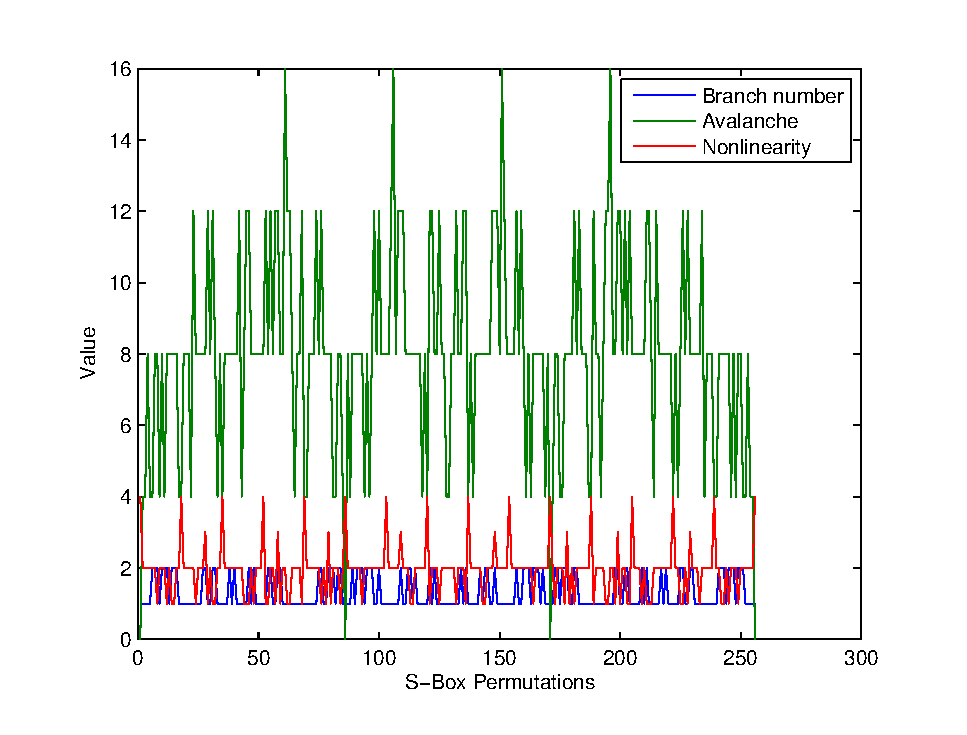
\includegraphics[scale=0.65]{images/brute_joint.eps} 

	\caption{The results for the branch number, avalanche number, and degree of nonlinearity for a $2$-bit S-box over all possible permutations in the design variables. Note that there are $4^4 = 256$ possible permutations over the S-box configuration permutation space because each element $x \in \field{F}_2^2$ can map to any output value $y \in \field{F}_2^2$.}
	\label{bfjoint}
\end{figure}
Exhaustive searches over the entire S-box permutation design space have a time complexity of $O(n^n)$ and thus are only feasible for very small order S-boxes. However, recent research efforts have advanced the upper bound on these exhaustive searches to include $4$-bit S-boxes, which were run in \cite{Sbox4x4}. Unfortunately, measurements for the branch number, avalanche number, and nonlinearity degree were not provided. 

As an alternative to performing these brute force searches, we consider the problem of optimizing the branch number, avalanche number, and degree of nonlinearity of symmetric-key cryptographic algorithm as MINLP problems, which can be formulated as shown in Figure \ref{problems}. It is important to note that the design variables for these problems correspond to the S-box configuration (i.e. the mapping of the function).

\begin{figure}[!ht]

\centering
\shadowbox{%
\parbox{15cm}{% 
\textbf{Branch Number - Minimize}
\begin{eqnarray*}
B_N'(X) = -B_N(X) = -\text{min}_{i, j\not=i}(\text{wt}(i \oplus j) + \text{wt}(X(i) \oplus X(j))),
\end{eqnarray*}
subject to the constraints
\begin{eqnarray*}
0 \leq X(i) & \leq & 2^{n} - 1 
\end{eqnarray*}
where $n$ is the number of bits needed to represent the design variables.
}}
%\end{figure}
\vspace{0.5cm}

%\begin{figure}[!ht]
%\centering
\shadowbox{%
\parbox{15cm}{% 
\textbf{Avalanche Number - Minimize}
\begin{eqnarray*}
A_N'(X) = -A_N(X) = -\sum_{i = 0}^{n - 1}\sum_{x \in \field{F}_2^n} \text{wt}(f(x) \oplus f(x \oplus 2^{i}))
\end{eqnarray*}
subject to the constraints
\begin{eqnarray*}
0 \leq X(i) & \leq & 2^{n} - 1 \\
\sum_{i = 0}^{n - 1}\sum_{x \in \field{F}_2^n} \text{wt}(f(x) \oplus f(x \oplus 2^{i})) - n^22^{n-1} & \leq & 0
\end{eqnarray*}
where $n$ is the number of bits needed to represent the design variables. 
}}
%\end{figure}
\vspace{0.5cm}

%\begin{figure}[!ht]
%\centering
\shadowbox{%
\parbox{15cm}{% 
\textbf{Degree of Nonlinearity - Minimize}
\begin{eqnarray*}
P_S(X) = \text{max}_{0 \not= a, b}|\{x \in \field{F}_2^n : S(x + a) - S(x) = b\}|,
\end{eqnarray*}
subject to the constraints
\begin{eqnarray*}
0 \leq X(i) \leq 2^{n} - 1,
\end{eqnarray*}
where $n$ is the number of bits needed to represent the design variables. 
}}
\caption{MINLP optimization problem definitions for the branch number, avalanche number, and nonlinearity degree measurements. It is important to note that the lack of additional constraints on these objective functions is intentional. Due to the nature of S-boxes and their application inside cryptographic algorithms, additional constraints might serve as additional information for attackers to exploit. }
\label{problems}
\end{figure}

\section{Candidate MINLP Optimization Algorithms}
%1. GA description - TODO: write up some characteristics of this algorithm
%2. BB description - TODO: write up some characteristics of this algorithm

Analyzing the function values for the branch number, avalanche number, and degree of nonlinearity over the S-box permutation design space indicates that each function is highly unstable and discontinuous. Therefore, traditional optimization methods that rely on the continuity of the functions are not likely to be very effective when solving these optimization problems. This section discusses some potential optimization algorithm candidates and describes why a genetic algorithm was chosen as the desired solution approach.

\subsection{Traditional Optimization Algorithms}
%4. discuss why BB algorithm didn't work (converged too early and didn't exhaust, too many local minimums for every objective function, GA was good because it generated populations and did psuedo brute force thing)

The \emph{Branch and Bound} algorithm is a very common optimization algorithm that is used to solve MINLP problems. In essence, it enumerates all candidate solutions for a given objective function and then uses the constraints to discard large portions of this collection at each iteration. However, this method is not suitable in the context of this problem for a variety of reasons. Firstly, the branch and bound approach is greedy in that it selects the appropriate decision branch to take to proceed towards the optimal value based on the current configuration. While this leads the algorithm towards an optimum value, it is usually a locally optimal solution. Furthermore, there is no penalty applied to the decision process that enables the design variables to change. Secondly, as shown in Figure \ref{bfjoint}, there are many locally optimum values for each objective function even with small order S-boxes. The usefulness of the BNB algorithm will surely degrade as larger order S-boxes are considered, because the number of intermediate local optimum values will increase significantly as well. This would cause the algorithm to converge to an optimal value too quickly and terminate with very few iterations. 

\subsection{Evolutionary Optimization Algorithms}

Given the instability of each of these functions over the permutation design variable space, it is natural to solve these MINLP problem using a probabilistic optimization algorithm. For the purposes of this project, the main results were derived using a highly probabilistic genetic algorithm that attempts to explore the configuration permutation space as much as possible in search for the global optimum values. Genetic algorithms are commonly utilized in the context of cryptography to explore the design space for cryptographic functions. This is primarily because they serve as an intelligent optimization method that can ease the computational efforts of performing brute force searches among the design space, which is crucial for functions with larger domains \cite{Skein}.

In this project, the genetic algorithm was configured in a very particular way to yield the optimal S-box configurations. Specifically, each objective function was set to the solver fitness function. In addition, the population generation and mutation steps in the algorithm were randomized so as to avoid early convergence to local optimal solutions for each fitness function. Also, the crossover function was entirely removed from the solver, which meant that the only design variable change came from the mutation function. This was done so as to place more control over the population generation. 

\begin{comment}
Since each of the aforementioned objective functions exhibit the same instable behavior, it is possible to apply the same genetic algorithm structure to solve each one of these. In particular, the genetic algorithm configuration for each of these problems used the following parameters.

\begin{table}
	\centering
	\caption{Genetic algorithm configuration parameters.}
    \begin{tabular}{|l|l|}
        \hline
        \textbf{Algorithm Option} & \textbf{Configuration Description} \\ \hline
        Population mutation function & Randomly scale each design variable based on the current generation \\ 
        Generations & $500$ \\ 
        Tolerance Function limit & $1 \times 10^{-6}$ from last function value change \\ 
        Stall generation limit & $2^{n^n}$ identical function values \\ 
        Initial population & S-box configuration $\langle 0, 1, ..., n \rangle$ \\
        \hline
    \end{tabular}
	\label{configTable}
\end{table}
\end{comment}

\section{Genetic Algorithm Optimization Results}
%TODO: compare GA results against exhaustive search and BB algorithm
%1. prsent individual and joint results for order 8 and 16  (3-bit and 4-bit S-boxes)
%2. discuss how close they got to optimal results
%3. discuss usefulness of GA
%4. discuss why BB algorithm didn't work (converged too early and didn't exhaust, too many local minimums for every objective function, GA was good because it generated populations and did psuedo brute force thing)

We now present the optimization results from the genetic algorithm solver for the three objective functions listed in the Section 2 for $3$- and $4$-bit S-box configurations. Each objective function is first optimized individually and then they are joined together as a multi-objective MINLP problem. 

Also, since the genetic algorithm sovler is a probabilistic algorithm that randomizes the population at each generation, it is important to note that each algorithm was run many times to obtain the optimal results. Due to the highly unstable objective functions, it is not enough to run the algorithm once and conclude that the results are optimum. 

\subsection{Avalanche Number}

From Section \ref{strength} we know that the optimal value for the avalanche number of an $n$-bit S-box is $n^22^{n-1}$. Therefore, for $3$- and $4$-bit S-boxes, we conclude that the optimal values are $3^2(2^2) = 9(4) = 36$ and $4^2(2^3) = 16(8) = 128$, respectively, since we are concerned with the avalanche effect over every single bit. Now, we compare these optimal values against those obtained from the optimization algorithm. Table \ref{avTable} contains the optimal results for a $3$-bit S-box configuration that were collected over a variety of optimization runs, and Figure \ref{av16} contains a diagram of the best iteration pattern of the algorithm for a higher order $4$-bit S-box configuration. 

Based on these results we can see that the genetic algorithm was able to reach an optimal value of $30$ for the $3$-bit S-box, which is approximately $16\%$ away from the global optimal value of $36$. Similarly, the genetic algorithm was able to reach an optimal value of $96$, which is approximately $25\%$ away from the global optimal. We also note that these results were achieved with relatively high coverage of the configuration space (as indicated by Figure \ref{av16}).

Clearly, we see that the accuracy of the genetic algorithm decreases as the order of the S-box gets higher. This is most likely due to the fact that the function for the avalanche number is very unstable and contains many local optimal values, and even with a probabilistic population generation procedure it is difficult to explore beyond one of these local optimal values. However, given the time complexity difference between the exhaustive search and the genetic algorithm solver, this may be a reasonable compromise in terms of security if a better configuration cannot be found manually. 

\begin{table}
	\centering
	\label{avTable}
	\caption{Some results from the genetic algorithm solver for the avalanche number of $3$-bit S-boxes.}
    \begin{tabular}{|l|l|l|}
        \hline
        S-Box Configuration & Optimal Function Value & Generations \\ \hline
        6     1     1     2     1     6     6     1 & 30 & 63 \\
        6     1     5     6     1     6     2     1 & 28 & 58 \\ 
        6     1     3     6     3     6     4     1 & 26 & 57 \\ 
	6     3     3     4     2     5     5     2 & 22 & 63 \\ 
        0     7     7     4     6     1     1     2 & 20 & 51 \\ 
        \hline
    \end{tabular}
\end{table}

\begin{figure}[!ht]
\centering
	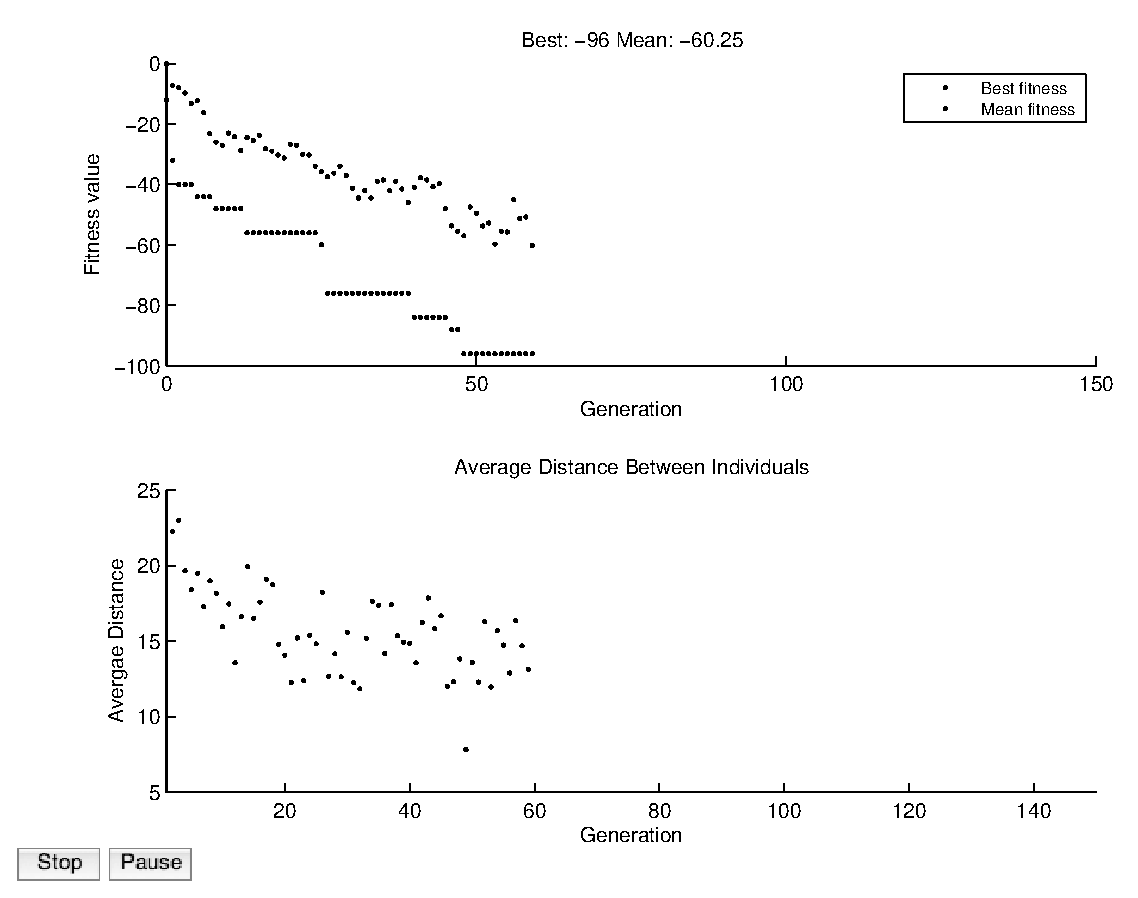
\includegraphics[scale=0.5]{images/avalanche_results16.eps} 

	\caption{A single evolution of the optimal solution to the avalanche number of a $4$-bit S-box configuration with a maximum of $500$ generations. Note that the solver converged to a sub-optimal result after computing $60$ generations, which is an indication that the solution reached a locally optimal solution.}
	\label{av16}
\end{figure}

\subsection{Branch Number}

%http://www.iacr.org/archive/fse2006/40470042/40470042.pdf - shows that branch number is maximum if %q+1 (order of field + 1?) Give the equation and then show that this does not produce optimal results.
%\cite{MaxBN}

It has been proven that the maximum branch number for an $n$-bit S-box is equal to $n$ \cite{MaxBN}. Therefore, in the case of $3$- and $4$- bit S-boxes, we know that the maximum possible branch numbers are $3$ and $4$, respectively. Given the small permutation design space for the $3$-bit S-boxes, the genetic algorithm solver was able to obtain this optimal value in only a small number of instances. The majority of the executions converged to the local optimal value of $2$, as shown in Table \ref{bnTable}.

\begin{table}
	\centering
	\label{bnTable}
	\caption{Some results from the genetic algorithm solver for the branch number of $3$-bit S-boxes.}
    \begin{tabular}{|l|l|l|}
        \hline
        S-Box Configuration & Optimal Function Value & Generations \\ \hline
        3     4     0     7     5     2     6     1 & 3 & 500 \\ 
	3     6     4     1     5     0     2     7 & 3 & 500 \\ 
        4     7     6     1     2     1     5     6 & 2 & 500 \\ 
        5     3     1     5     6     5     0     7 & 2 & 500 \\ 
        1     3     0     2     7     2     6     3 & 2 & 500 \\ 
        \hline
    \end{tabular}
\end{table}

Extending the order of the S-box to $4$ bits made the solver even less effective at finding the optimal value of $4$. As shown in Figure \ref{bn16}, although each generation covered a large area of the state space (as indicated by the average bit-wise distance between parents and children), the solution still converged to the local optimum of $2$ even after $500$ generations. In fact, there was no execution of the solver that yielded a higher value for the branch number, even with the high configuration space coverage (as indicated by the large variation in the average distance scatter plot).

This is an obvious result due to the instability of the branch number function over the configuration permutation state space. Since there are so many local optimal values for the function that increases with the order of the S-box, the solver simply converges to the nearest optimal and then orbits around that value for each of the following generations. Based on these results we conclude that the usage of a genetic algorithm is not particularly helpful when optimizing the branch number of S-boxes.

\begin{figure}[!ht]
	\centering
	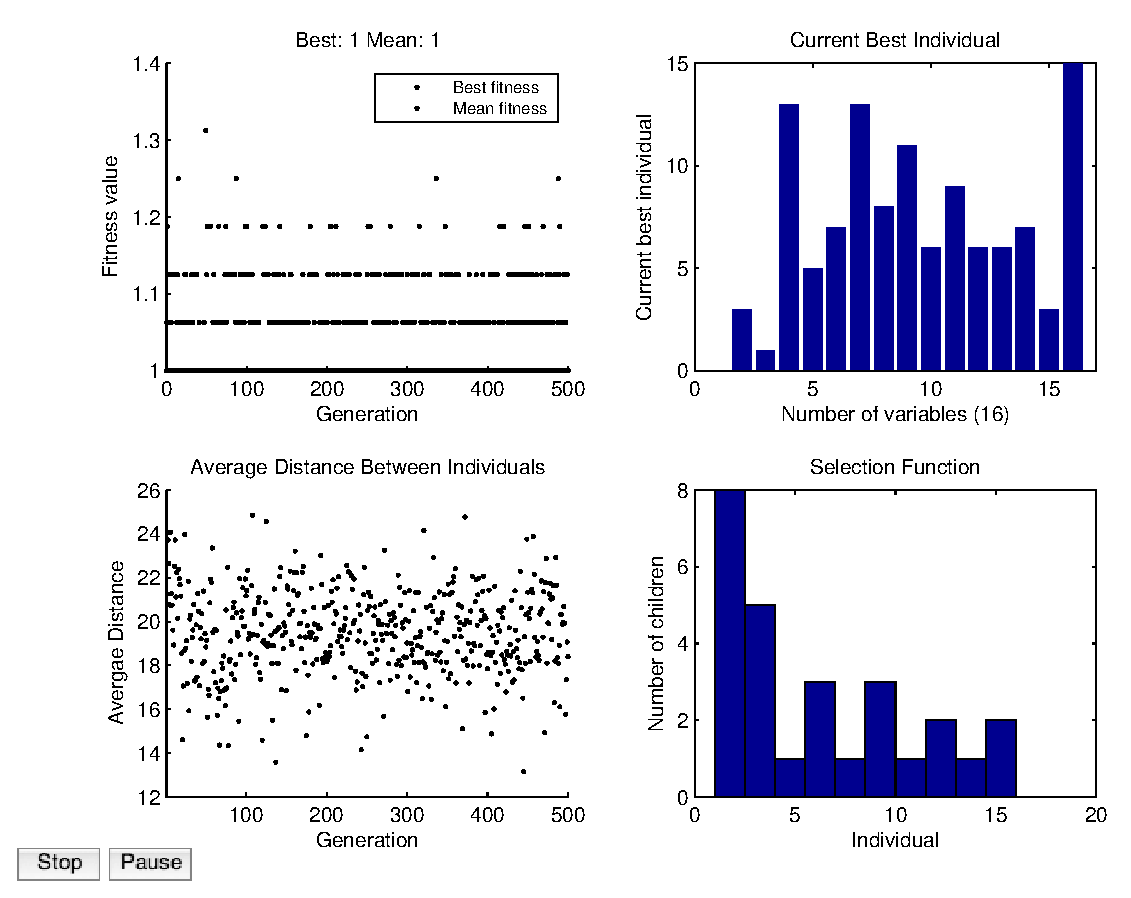
\includegraphics[scale=0.5]{images/bn_results16.eps} 

\caption{A single evolution of the solution to the branch number of a $4$-bit S-box configuration with a maximum of $500$ generations, which covered a large amount of the configuration space.}
	\label{bn16}
\end{figure}

\subsection{Degree of Nonlinearity}
It has been shown that the most optimal value for $P_S$ is $1$, meaning that the S-box is "perfectly nonlinear" in that it is resistant to any forms of differential cryptanalysis \cite{ProvableSecurity}. However, almost-perfect nonlinear (APN) S-boxes have also been studied extensively by Nydberg and are shown to be almost equally resistant to the most sophisticated differential cryptanalysis attacks, where $P_S \leq 2$ for such S-box configurations. Therefore, as shown in Table \ref{nlTable}, the genetic optimization solver was able to find a variety of S-box configurations qualify them as APN, which is an indication that the S-box is secure against common attacks. Unfortunately, the solver was not able to find a configuration that yielded the perfectly nonlinear configuration value of $P_S = 1$. 

\begin{table}
	\centering
	\caption{Some results from the genetic algorithm solver for the degree of nonlinearity of $3$-bit S-boxes.}
	\label{nlTable}
    \begin{tabular}{|l|l|l|}
        \hline
        S-Box Configuration & Optimal Function Value & Generations \\ \hline
        4     2     1     4     1     1     5     4 & 2 & 51 \\ 
        6     3     6     5     1     5     5     1 & 2 & 51 \\ 
        0     3     3     6     7     6     2     2 & 2 & 51 \\ 
        3     4     1     5     4     0     6     6 & 2 & 51 \\ 
        \hline
    \end{tabular}
\end{table}

Extending the order of the S-box to 16 elements and running the same test yielded similar APN results, as shown in Figure \ref{nl16}. The solver was able to converge to the optimal value of $2$ for in a relatively small number of generations, which is a good indication that the instability of the function does not deter the algorithm as significantly as it did with the branch number function. Based on these results, we can assume that this pattern would likely continue into higher order S-boxes, and thus we conclude that the genetic algorithm is very well suited to finding the S-box configuration that achieves an acceptable degree of nonlinearity.

\begin{figure}[!ht]
	\centering
	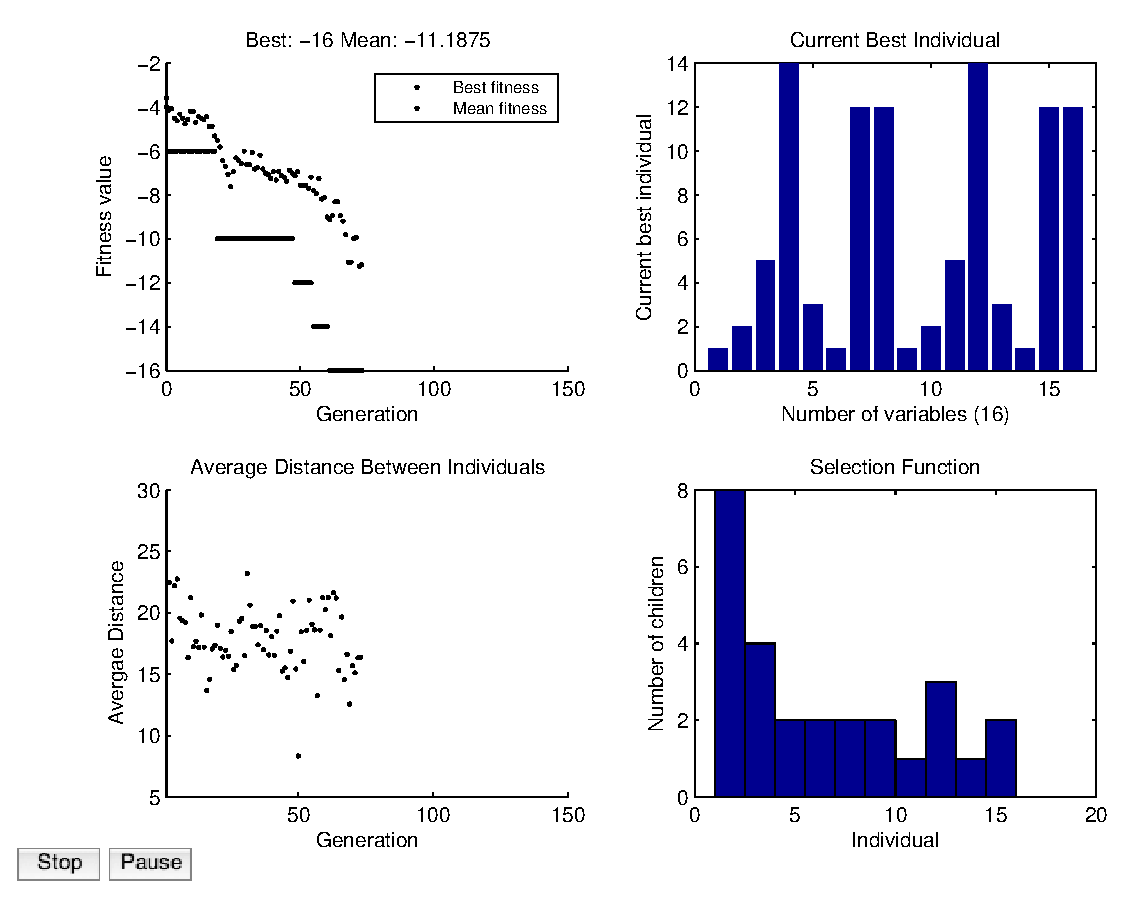
\includegraphics[scale=0.5]{images/nl_results16.eps} 

\caption{A single evolution of the optimal solution to the nonlinearity degree of a $4$-bit S-box configuration with a maximum of $500$ generations.}
	\label{nl16}
\end{figure}

\subsection{Multi-Objective Optimization}
Separately, the branch number, avalanche number, and degree of nonlinearity all contribute to the overall levels of confusion and diffusion of a symmetric-key cryptosystem. However, it is not enough to consider these problems separately because an optimal configuration for one measurement might not align with the optimal measurement for another. Therefore, it is ideal to find a shared solution S-box configuration that satisfies all three objective functions simultaneously. The most common way to solve this problem is to formulate the optimization problem as a linear combination of all three objective functions. The benefit of this approach is that we can prioritize the influence that each objective function has on the overall solution by assigning weights to each value in this linear combination. Such a linear combination is defined as $f(X) = w_1A_N'(X) + w_2B_N'(X) + w_3P_S(X)$, where $w_1, w_2$, and $w_3$ are not design variables. 

\begin{comment}
\begin{figure}[!ht]
\centering
\shadowbox{%
\parbox{15cm}{% 
\textbf{Joint MINLP Problem - Minimize}
\begin{eqnarray*}
f(X) = w_1A_N'(X) + w_2B_N'(X) + w_3P_S(X),
\end{eqnarray*}
subject to the constraints
\begin{eqnarray*}
0 \leq X(i) & \leq & 2^{n} - 1 \\
\text{min}_{i, j\not=i}(\text{wt}(i \oplus j) + \text{wt}(X(i) \oplus X(j))) - n2^{n-1} & \leq & 0,
\end{eqnarray*}
where $n$ is the number of bits needed to represent the design variables and $w_i$, where $1 \leq i \leq 3$, are \emph{not} design variables. 
}}
\caption{The joint MINLP problem formalization as a linear combination of all three objective functions under the same constraints.}
\label{jointProblem}
\end{figure}
\end{comment}

Since the weighted priorities of each objective function in this linear combination are values that should be tweaked by the cryptographer in response to their own security priorities, they are not treated as design variables in this problem. Based on the research that was conducted into each of these metrics, various weights were assigned to this expression and then run through the genetic algorithm solver to see if a shared optimal solution could be generated. A subset of the results for $3$-bit S-boxes is shown in Table \ref{jointTable}, and a single execution of the solver is shown in Figure \ref{joint16}.

\begin{table}
	\centering
	\caption{Sample linear weights and the corresponding function value tuples for the avalanche number, branch number, and degree of nonlinearity for $3$-bit S-boxes. The high weights on the branch number and nonlinearity degree selection comes from the need for higher measures of confusion (from nonlinear operations) than diffusion (from linear operations) in the S-box.}
	\label{jointTable}
    \begin{tabular}{|l|l|l|l|l|}
        \hline
        $w_1$ & $w_2$ & $w_3$ & S-Box Configuration & $(A_N, B_N, P_S)$ \\ \hline
        1 & $2^8$ & $2^8$ & 5     6     2     5     5     6     2     5 & (40, 1, 8) \\ 
        1 & $2^4$ & $2^8$ & 4     3     3     6     2     5     5     4 & (50, 1, 6) \\ 
        1 & $2^8$ & $2^4$ & 2     5     2     2     2     5     2     2 & (24, 1, 8) \\ 
        1 & $2^4$ & $2^4$ & 3     5     4     2     3     5     4     2 & (40, 1, 8) \\ 
        \hline
    \end{tabular}
\end{table}

Based on these results, it is clear that each of the objective functions in this linear combination do in fact interact destructively when combined to form the overall objective function. This claim is supported by Figure \ref{bfjoint}. The immediate implication of this is that any change in the population is likely to improve one objective function at the expense of degrading another. As the simulation in Figure \ref{joint16} indicates, even with large significant changes in the children after every generation of the genetic algorithm, the joint objective function tends to stay at the same optimal value because of the degrading penalty suffered by such changes. Therefore, we conclude that the genetic algorithm is not an effective technique for exploring the configuration permutation space and trying to optimize all three objective functions together at once. 

%\begin{comment}
\begin{figure}[!ht]
	\centering
	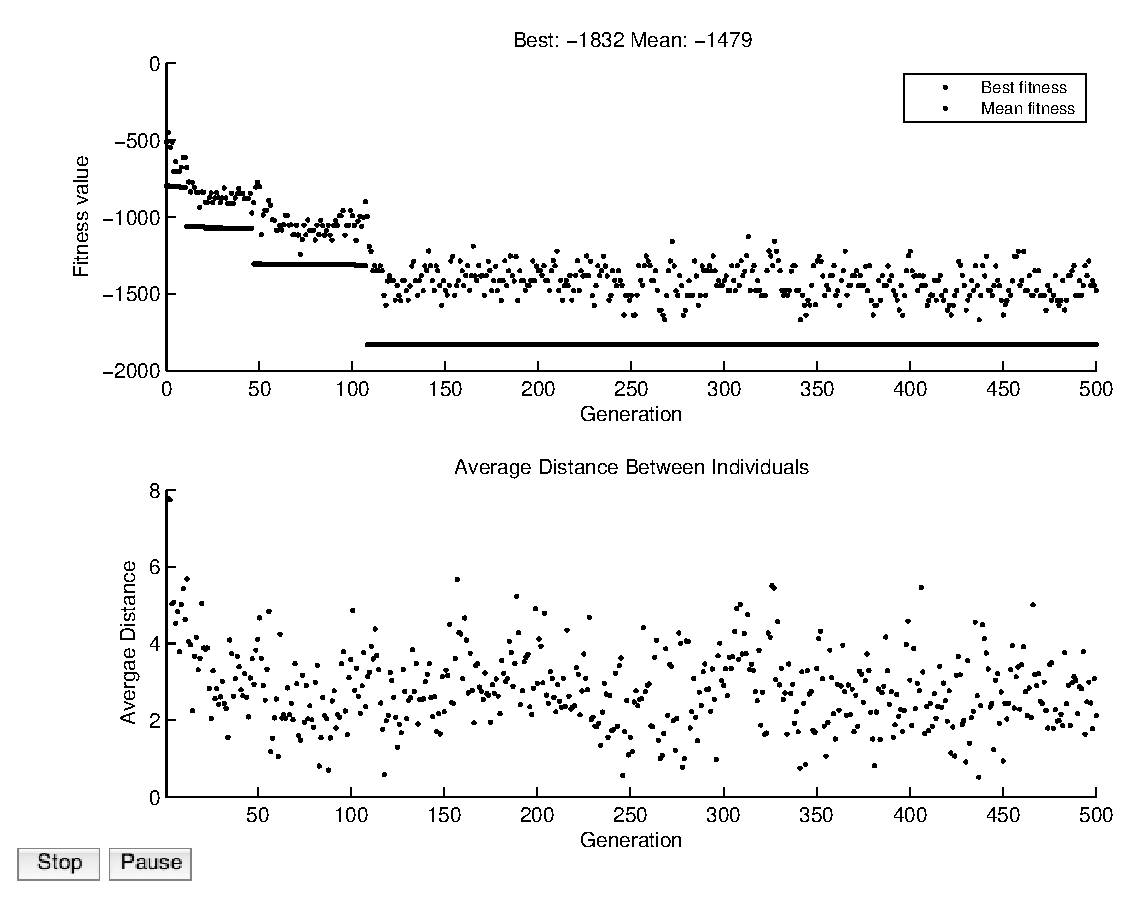
\includegraphics[scale=0.5]{images/joint_results16.eps} 
	\label{joint16}
\caption{A single evolution of the optimal solution to the joint objective fucntion of a $3$-bit S-box configuration with a maximum of $500$ generations, where the weights are $1$, $2^8$, and $2^8$, respectively.}
	\label{joint16}
\end{figure}
%\end{comment}

% http://www.reveresecurity.com/_pdfs/s4x4Analysis.pdf
% says that BN must be at least 2 for bijective S-boxes

\section{Conclusions}
%TODO: GA was most promising - similar to BF approach
%TODO: results were closest to brute force, and presumed to be close to actual values
%TODO: joint computations using GA were ineffective, exhaustive searches would be better, contradicting functions caused too great penalties and little change in design variabes
%TODO:  GA work - tweak crossover and mutation functions, run on large scale hardware/software systems

Based on the results from the individual optimization problems and combination problem, we can conclude that the use of genetic algorithms (or any evolutionary algorithm) have very limited or specialized use in the context of cryptography. Most cryptographic functions (and even measurements of those functions) are truly random across the function domain, and this seemingly random behavior leads to discontinuous and instable functions with many local optimal solutions. While this rules our traditional optimization algorithms that rely on the smoothness of functions almost immediately, it still leaves some room for probabilistic evolutionary algorithms. 

However, as was shown, the application of such evolutionary algorithms is only moderately useful when optimizing a single dimension (or measurement) of cryptographic algorithms; it is not effective when optimizing multiple dimensions at once. The reason for this is that when superimposing each of these functions on top of one another we are left with a great deal of destructive interference. That is, improvements in one objective function are very likely to degrade the value of another objective function.

Since cryptographers seek to optimize multiple dimensions at once, the application of such optimization algorithms is likely yield little or no significant benefits. This conclusion supports the lack of research done in this problem in the field of cryptography. However, that is not to say that the application of all evolutionary algorithms should be ruled out altogether. Perhaps as researchers further refine the security measurements for symmetric-key cryptosystems we may be able to define a multi-objective MINLP that can be optimized to find an optimal configuration for S-boxes. However, until that time, we are left with intuition and mathematical derivations for optimal S-box configurations.

\bibliographystyle{IEEEtran}
% argument is your BibTeX string definitions and bibliography database(s)
\bibliography{caw4567-report-final}

\end{document}
